\documentclass{article}
\usepackage{graphicx}
\bibliographystyle{plos2009}

\begin{document}

\title{Isolation of a {\em Shewanella} species that grows
  anaerobically on nitrate and acetate and aerobically on LB}
\author{C. Titus Brown}
\date{August 15, 2016}

\maketitle

\section*{Introduction}

My initial interest was in isolating and studying sulfur-oxidizing
denitrifying autotrophs in the environment and comparing their
metabolic versatility to that of {\em Sulfuromonas denitrificans}
\cite{sievert2008genome}.  However, we instead enriched for nitrate-
and acetate-dependent organisms that are almost certainly
heterotrophs.

\section*{Methods and Data}

\paragraph{Isolation media} Isolation media was concocted as follows:
First, ``brackish base'' (BB) was made by combining a number of salts
(Table~\ref{tab:media}) per liter final volume and autoclaving to
sterilize.  Then, sodium bicarbonate and potassium phosphate (5g
NaHCO$_3$ and 0.5g KH$_2$PO$_4$) were dissolved in 50ml H$_2$O,
sterile filtered, and added, along with 1ml sterile filtered trace
metal solution (JRL 2016 special sauce).

To this base BB media, one or more of sterile-filtered 10 mM
thiosulfate (``S''), 20 mM potassum nitrate (``N''), and/or 10 mM
sodium acetate (``A'') was added as described below.

To make plates, 1 gram-percent agar was added to the basic solution.

\begin{table}
\centering
\begin{tabular}{|c|c|}
\hline
Amount & Chemical \\
\hline
10.5g & NaCl \\
1.7g & MgCl$_2$.6H$_2$O \\
0.125g & CaCl$_2$.2H$_2$O \\
0.5g & KCl \\
\hline
\end{tabular}
\caption{BB base media salts}
\label{tab:media}
\end{table}

\paragraph{16s Colony PCR} Each colony was picked and touched to 20ul of
alkaline PEG200 (``ALP'').  This was then boiled for 5 minutes to lyse
the cells. 1 ul of cell lysate was then added to a 25 ul Promega GoTaq
G2-based PCR reaction with the bacterial 16s primers 8F and 1391R.  16
rounds of PCR was performed with a 1.5 minute extension time.  After
PCR, bands were checked on a gel; then,
Sanger sequencing was performed directly from the PCR reactions with
the primer 515F.

\paragraph{Data availability}

All data is available at https://github.com/ctb/2016-micdiv-report/.

\section*{Results and Discussion}

\subsection*{An enrichment from Trunk River grew with the addition of acetate}

I initially designed media to enrich for sulfur oxidizing denitrifiers
(``BB+SN'').  I inoculated two Pfennig bottles (approx. 40ml)
with approximately 2-3 cc of material.  The material for the first
enrichment, culture 4, was taken directly from the sediment layer on
top of the sand in the main channel of Trunk River, approximately 8m
from the start of the narrow outflow channel. The material for the
second enrichment, culture 8, was taken from the underwater surface of
a sea table enrichment that originated from a microbial mat, also
taken from Trunk River.  Both enrichments were incubated at 30 deg
in a foil-lined box to prevent phototroph growth.

After 18 hours, significant turbidity was observed in both
enrichments, along with substantial amounts of supersaturated gas,
indicating growth.  I therefore transferred 1 ml from each enrichment
to another Pfennig bottle containing BB+SN.  These transfer
enrichments, however, failed to grow.

Based on scent, Dr. Leadbetter suspected that the original transfer of
sediment contained acetic acid, indicating the presence of significant
amounts of acetate.  I therefore added 400ul of 1M sodium acetate to
both enrichment cultures, to a final concentration of 10 mM.

After the addition of acetate, both transfers grew to white opacity
within about 16 hours at 30 deg.  Two subsequent transfers of each
culture (1ml into 40 ml ``BB+SNA'', BB with thiosulfate, nitrate, and
acetate) also exhibited similar growth.

\subsection*{Enrichments exhibited nitrate and acetate dependent growth}

To further analyze growth conditions, I employed a simple
``differential diagnosis'' approach and transferred each enrichment to
four culture conditions: BB, BB with thiosulfate and acetate (BB+SA),
BB with nitrate and acetate (BB+NA), and BB with acetate (BB+A).
After incubation for 16 hours, only the BB+NA cultures grew, indicating that
the enrichments required both nitrate and acetate but did not require
thiosulfate (Figure~\ref{fig:diff}).

\begin{figure}[!ht]
  \centerline{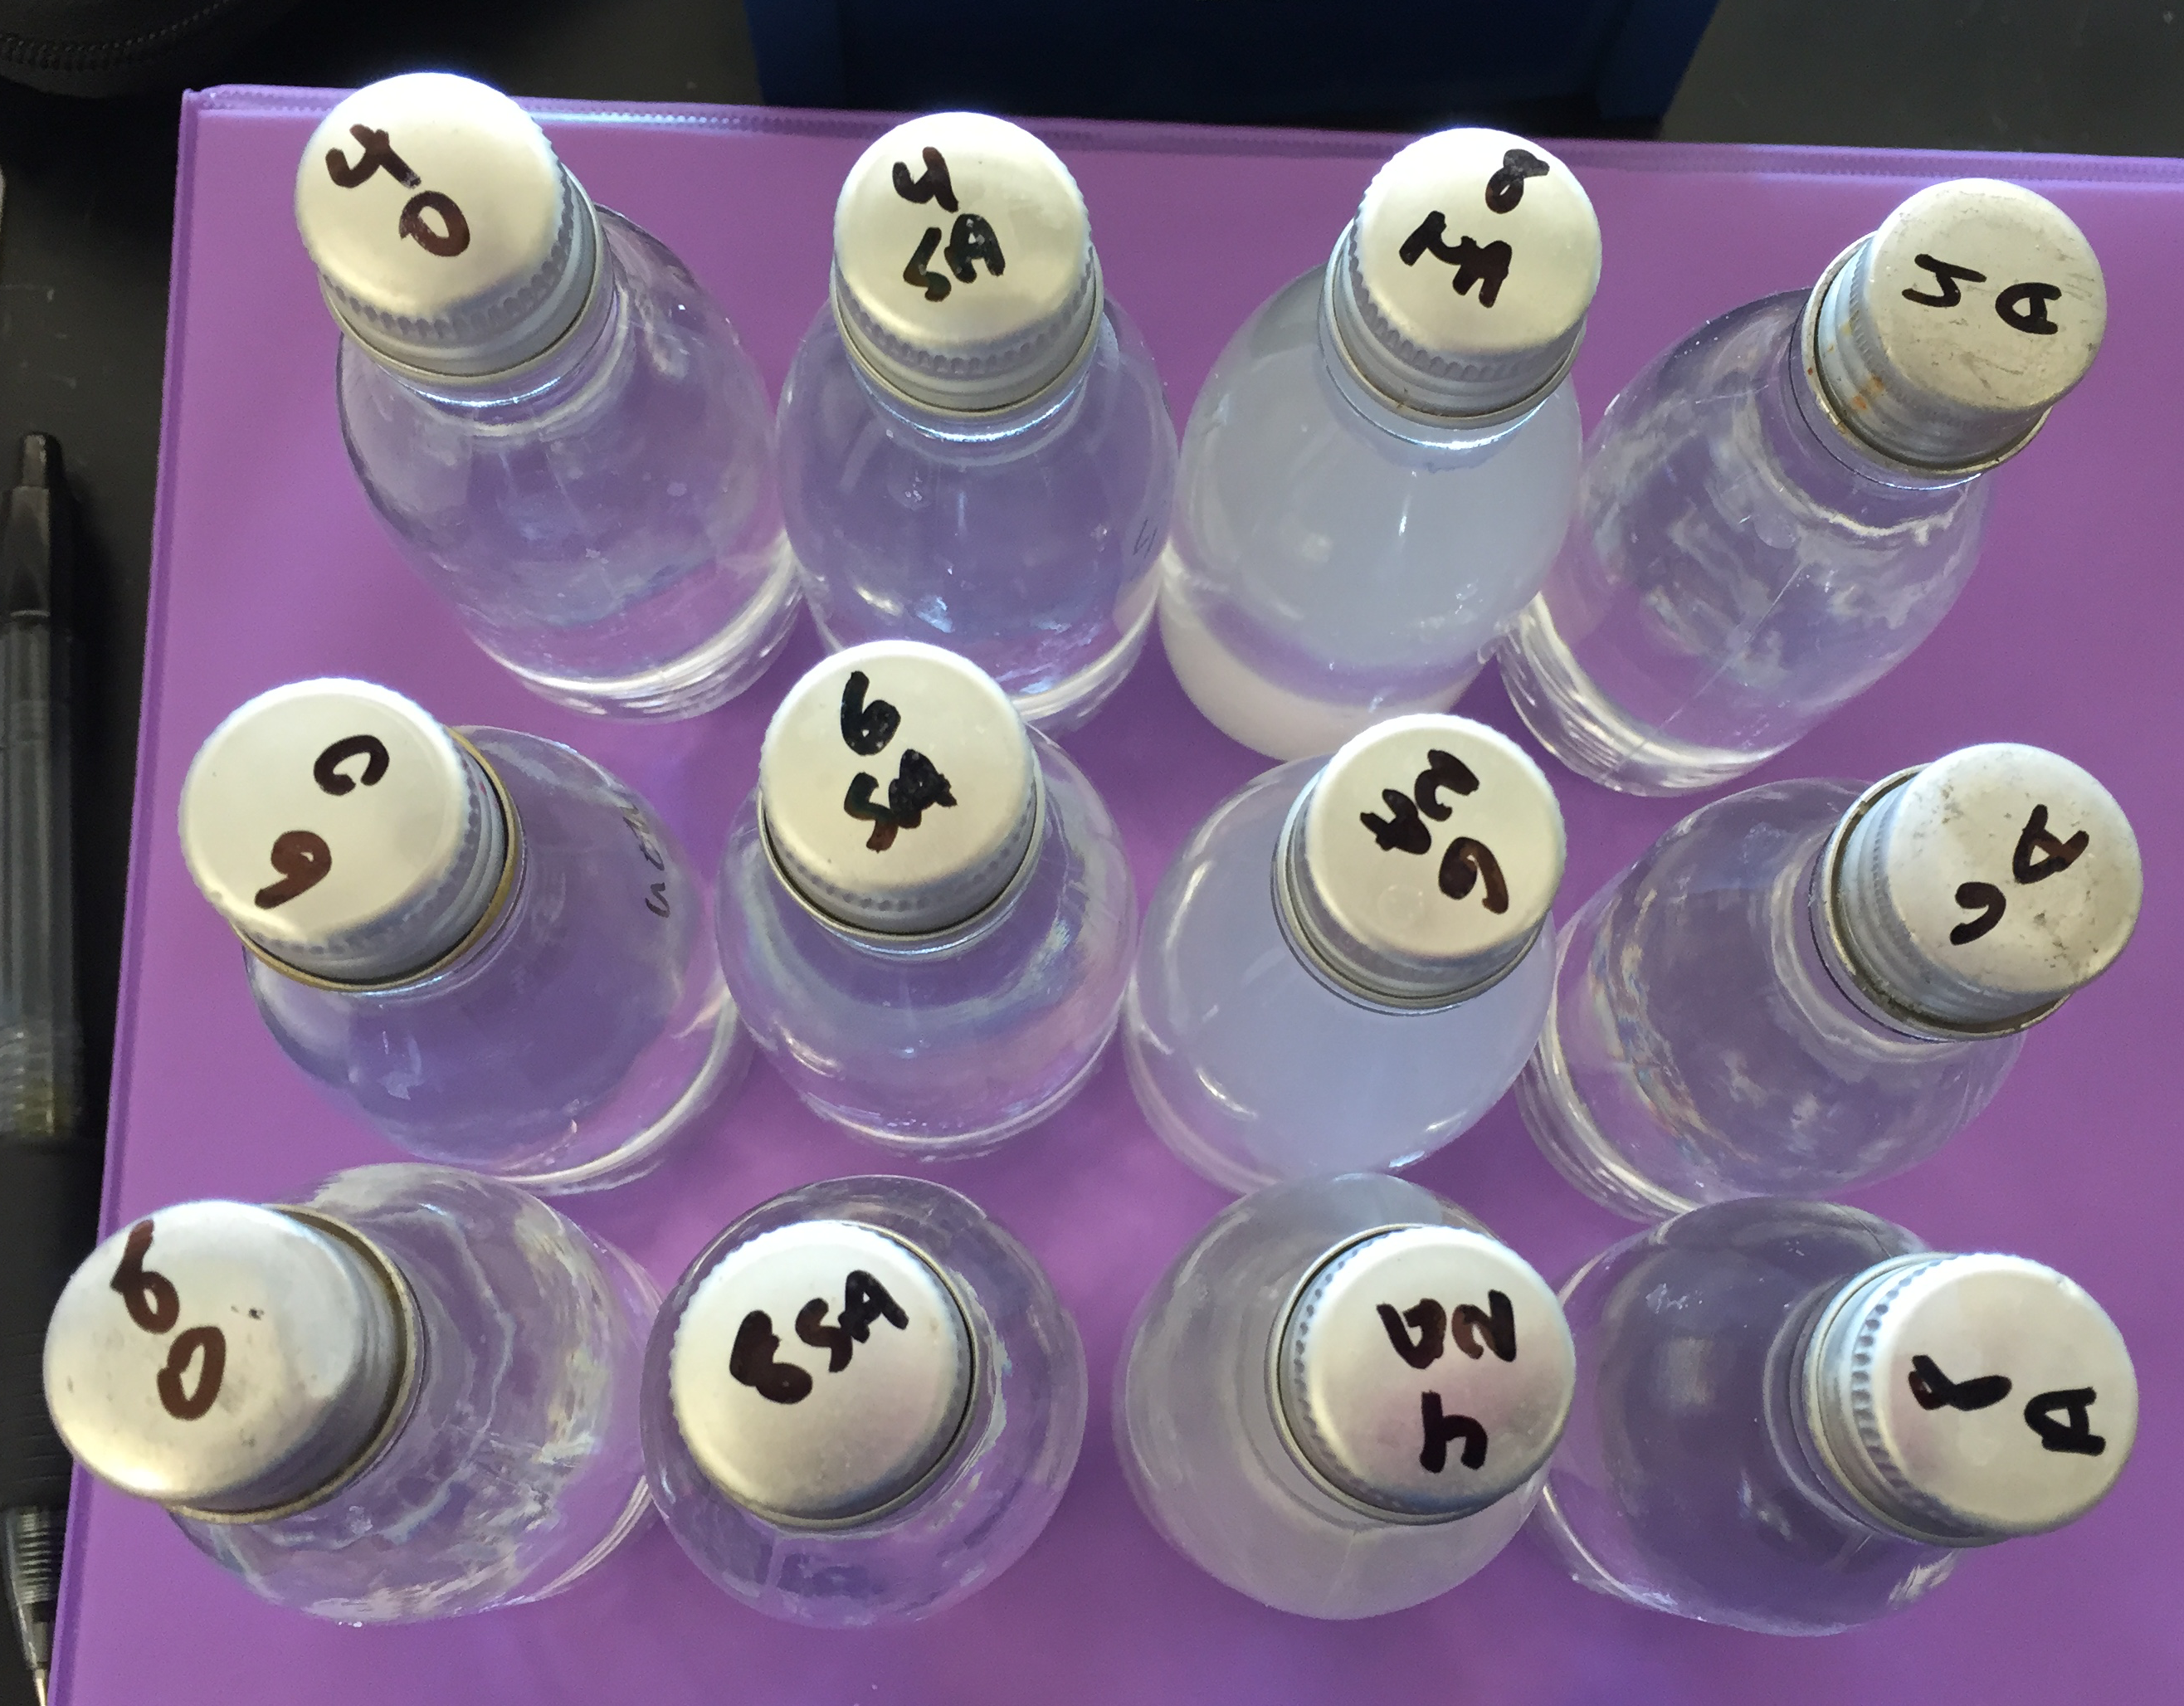
\includegraphics[width=4in]{diff.png}}
  \caption{Both enrichments 4 and 8 (first and third row) exhibit
    nitrate and acetate-dependent growth (third column) in anaerobic BB medium. No growth was observed in base BB media, BB+thiosulfate and acetate, or BB+acetate alone.}
  \label{fig:diff}
\end{figure}


\subsection*{Enrichments yielded colonies when grown on solid media}

I plated 1:500 and 1:5000 dilutions of enrichments 4 and 8 on BB+SNA
solid media, and incubated the plates both anaerobically and
aerobically at 30 deg.  I also plated the same dilutions on LB and
grew aerobically at 30 deg.  All plates showed density-dependent growth,
although the colonies on the LB plates grew much faster (2-4 times)
than either the aerobic or anaerobic BB plates.

\subsection*{Isolate colonies from aerobic LB plates grew successfully
  in anaerobic culture}

I picked 4 colonies grown aerobically on LB from each enrichment (for
a total of 8), and inoculated anaerobic BB+SNA cultures with them.
7/8 of the cultures grew within 48 hours, with three (culture 3 from
enrichment 8, and cultures 5 and 8 from enrichment 4) growing
overnight to opacity.

I then transferred these three isolates (3, 5, and 8) from BB+SNA
anaerobic liquid culture back to LB plates, where they again grew
(see Figure~\ref{fig:LB}).

\begin{figure}[!ht]
  \centerline{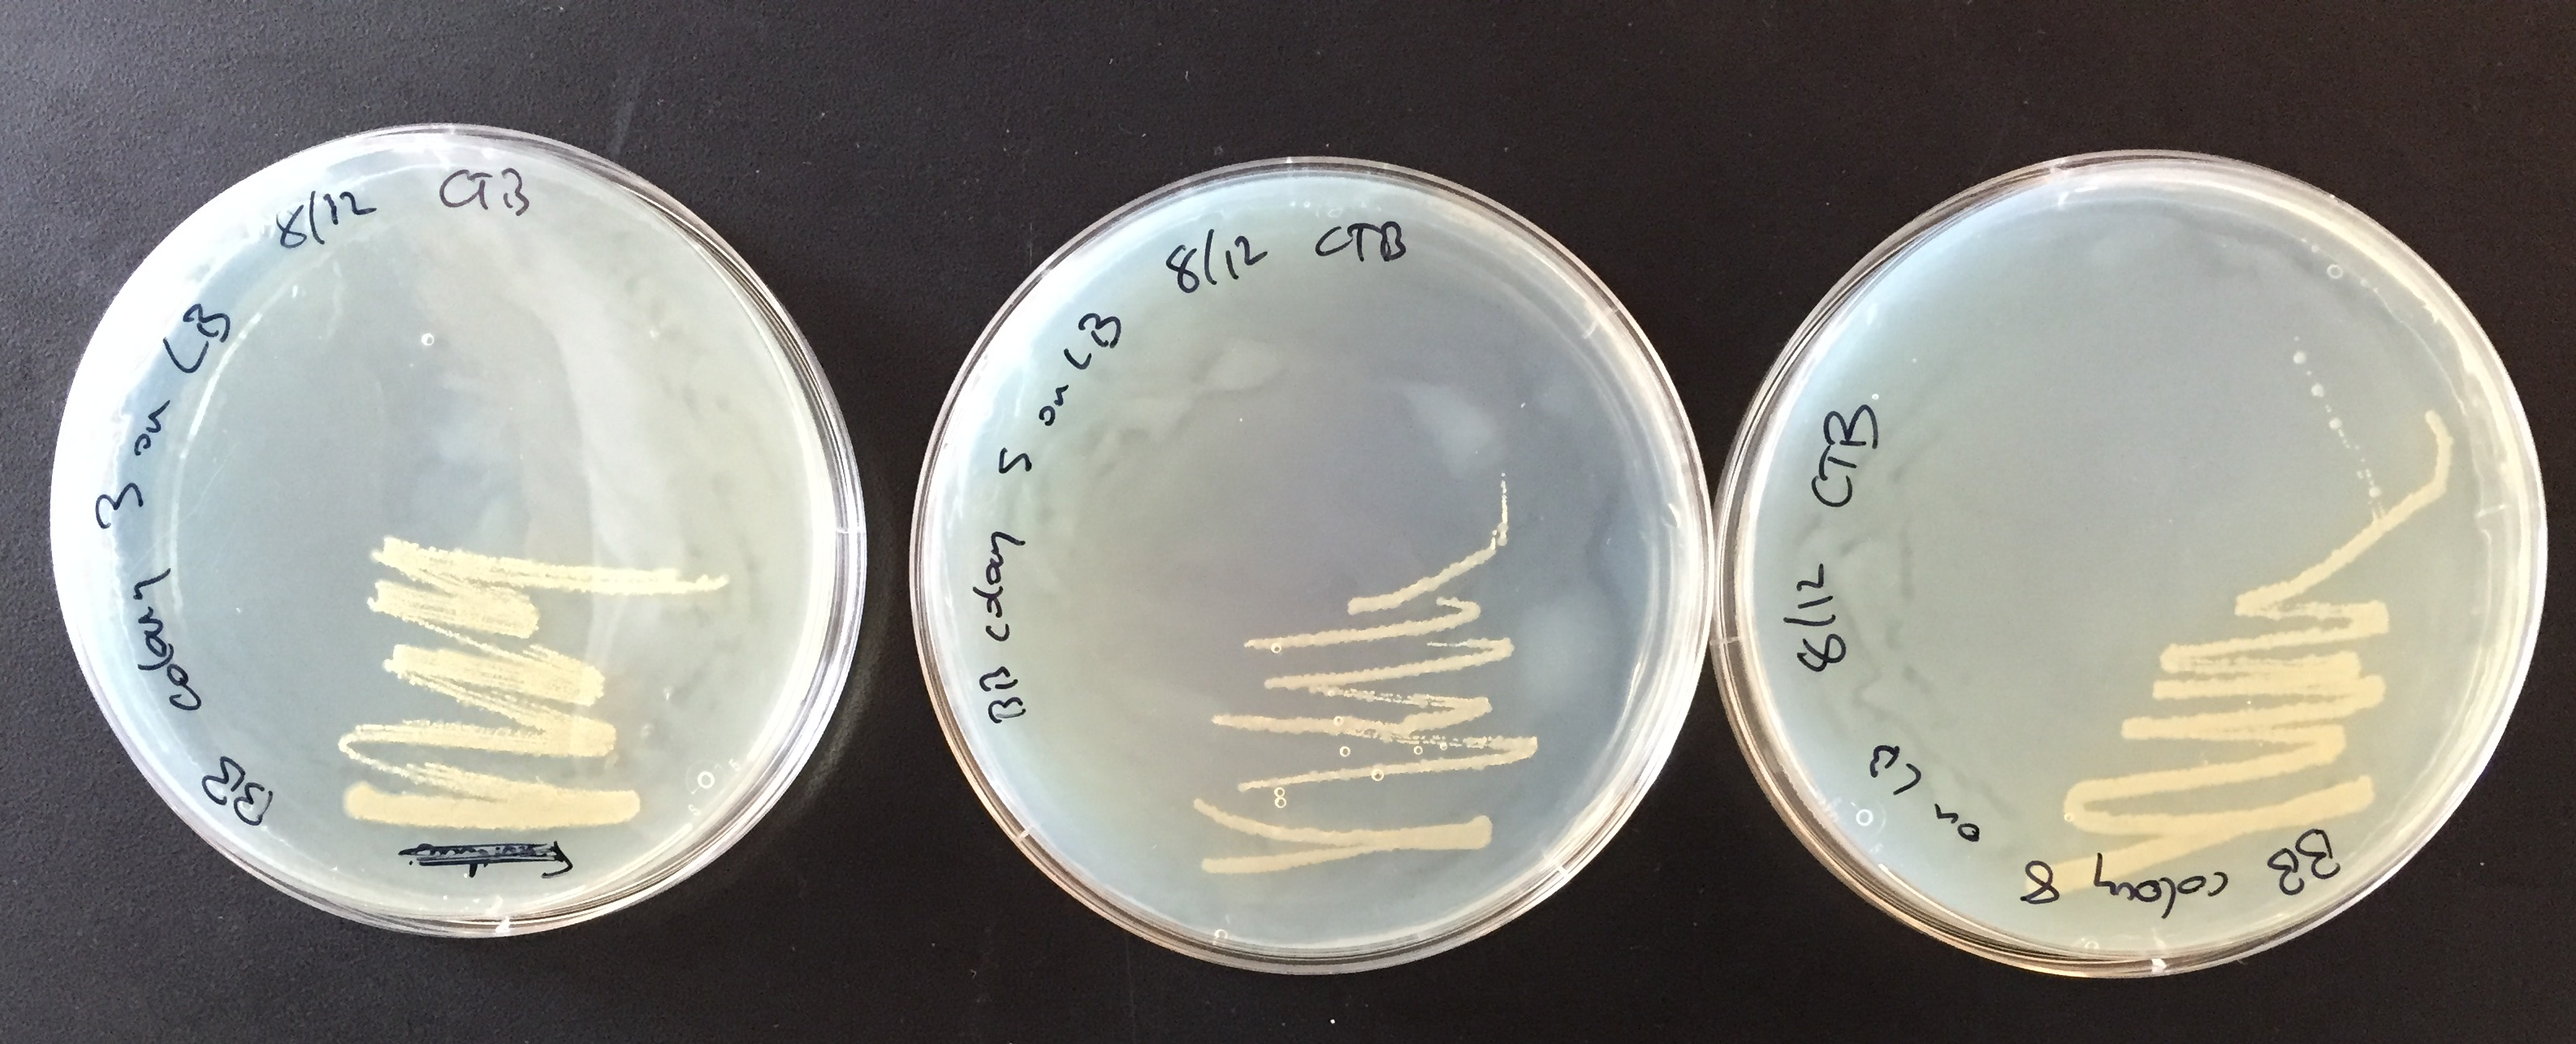
\includegraphics[width=4in]{LB.png}}
  \caption{All three isolate colonies grew after transfer from LB
    through BB+SNA anaerobic culture followed by streaking on LB.}
  \label{fig:LB}
\end{figure}

\subsection*{Isolate colonies were identified by 16s colony PCR as {\em Shewanella} spp.}

I picked colonies and performed 16s PCR on the eight LB isolate
colonies as described in the Methods.  All 8 yielded bands, which were
then Sanger sequenced.  BLAST of all 8 colonies against NCBI's ``nt''
database primarily recovered 16s sequences from {\em Shewanella}; the
best hits showed strong similarity (99\%) to two species of
{\em Shewanella} (Table~\ref{tab:16s}).

\begin{table}
\centering
\begin{tabular}{|c|c|c|l|l|}
\hline
Enrichment & Colony & Match percentage & BLAST match & Accession \\
\hline
1 &
8 &
99\% &
{\em Shewanella} algae strain MAS2736 &
GQ372874.1 \\

2 &
8 &
99\% &
{\em Shewanella} algae strain MAS2736 &
GQ372874.1 \\

3 &
8 &
99\% &
{\em Shewanella} algae strain MAS2736 &
GQ372874.1 \\

4 &
8 &
99\% &
{\em Shewanella} algae strain MAS2736 &
GQ372874.1 \\

5 &
4 &
99\% &
{\em Shewanella} sp. Chr-15 &
JQ863373.1 \\

6 &
4 &
99\% &
{\em Shewanella} sp. Chr-15 &
JQ863373.1 \\

7 &
4 &
99\% &
{\em Shewanella} sp. Chr-15 &
JQ863373.1 \\

8 &
4 &
99\% &
{\em Shewanella} sp. Chr-15 &
JQ863373.1 \\
\hline
\end{tabular}
\caption{BLAST-based characterization of Sanger-sequenced 16s regions from colony PCRs.  All colonies are clearly identified as {\em Shewanella} at 99\% identity.}
\label{tab:16s}
\end{table}

\subsection*{Isolate cultures contain Spirilla-shaped microbes}

I examined all three cultures with light microscopy and saw
Spirilla-like bacteria (Figure~\ref{fig:spirilla}).  These bacteria
appeared to move in a corkscrew-like fashion.  This morphology is at
odds with their molecular identification as {\em Shewanella} spp, which are
typically rod-shaped bacilli.

\begin{figure}[!ht]
  \centerline{\includegraphics[width=4in]{spirilla.png}}
  \caption{Light microscopy image of isolate colony 8, showing a
    bent-rod shape characteristic of spirillae; all three isolate
    colonies (3, 5, and 8) exhibited identical morphology.}
  \label{fig:spirilla}
\end{figure}

\subsection*{Isolate cultures produce some N$_2$O and little to no methane.}

Gas was sampled from headspace in the Pfennig bottles, and analyzed
with both mass spectrometry (for N$_2$O) and gas chromatography (for
methane).  10-20 nanomoles of nitrous oxide were seen in 2cc of
headspace.  Only trace amounts of methane (below 1\%) were observed
for the three isolates.

\section*{Discussion}

We robustly recovered two species of {\em Shewanella} from two
enrichments sourced in Trunk River.  {\em Shewanella} species are
often facultative anaerobes and can utilize a diverse array of
electron acceptors and carbon sources
\cite{venkateswaran1999polyphasic}; our results agree.  Here we find
that our strains grow quickly and robustly both aerobically on LB
plates and anaerobically on artisanal brackish media intended to
select for sulfide oxidizers, nitrate reducers and acetate consumers.

As there is no genome yet available for these strains, my next
proposed step would be to sequence and assemble the genomes of both
strains and compare gene complements.  Genes present in both would
presumably be important for acetoclastic denitrification and should
be readily identifiable.

\subsection*{Acknowledgements}

I would like to thank Jared Leadbetter, Dianne Newman, Kurt Hanselmann,
Elise Cowley, Gray Chadwick, Kate Hargraves, Kyle Costa, Bonita Lam,
Kristina Garcia, Dmitri Meier, and Scott Dawson for assistance during
this project.

% @HPLC / IC?

\bibliography{micdiv}

\end{document}
